\documentclass{article}[a4paper,12pt]

\usepackage{ae,lmodern}
\usepackage[utf8]{inputenc}
\usepackage[french]{babel}
\usepackage[T1]{fontenc}

\usepackage{graphicx}
\usepackage{xcolor}
\usepackage{tikz}

\definecolor{fadred}{RGB}{222,60,80}
\definecolor{warmgrey}{RGB}{155,155,155}
\definecolor{cornflowerblue}{RGB}{70,138,217}
\definecolor{lightsage}{RGB}{184,233,134}
\definecolor{bananayellow}{RGB}{249,236,79}

\title{\vfill Documentation Fonctionnelle de l'application MoodTracker}
\author{Cano Guillaume}
\date{\today\vfill}

\begin{document}


\maketitle


\newpage
\renewcommand{\contentsname}{Sommaire}
\tableofcontents
\newpage

\section{Introduction}

Ce document présente les fonctionnalités de l'application MoodTracker.
MoodTracker est une application permettant de mémoriser son humeur du jour,
et de consulter l'historique de ses humeurs sur les sept derniers jours.
Nous appellerons :

\begin{itemize}
\item Activité principale : l'activité qui permet à l'utilisateur
  de sélectionner l'humeur du jour.
\item Activité d'historique: l'activité qui consiste à mémoriser et
  à afficher l'humeur des sept derniers jours de l'utilisateur.
\end{itemize}

\medskip

Cette application est conçue pour fonctionner sur les versions d'Android
supérieur où égal à la version 4.4.

\section{Fonctionnalités de l'activité principale}

L'activité principale permet à l'utilisateur de choisir son humeur du jour parmi
les cinq humeurs suivantes :

\begin{itemize}
\item[]\begin{tikzpicture}
  \draw[fill=bananayellow] (0,0) rectangle (0.2,0.2);
\end{tikzpicture} Très bonne humeur.
\item[]\begin{tikzpicture}
  \draw[fill=lightsage] (0,0) rectangle (0.2,0.2);
\end{tikzpicture} Bonne humeur.
\item[]\begin{tikzpicture}
  \draw[fill=cornflowerblue] (0,0) rectangle (0.2,0.2);
\end{tikzpicture} Humeur normale.
\item[]\begin{tikzpicture}
  \draw[fill=warmgrey] (0,0) rectangle (0.2,0.2);
\end{tikzpicture} Mauvaise humeur.
\item[]\begin{tikzpicture}
  \draw[fill=fadred] (0,0) rectangle (0.2,0.2);
\end{tikzpicture} Très mauvaise humeur.
\end{itemize}

L'utilisateur peut changer son humeur du jour en faisant un glissement de doigt
sur l'écran vers le haut ou vers le bas (voir la figure~\ref{listhumeur}) :
\begin{itemize}
\item Un glissement vers le haut (swipe up) affiche une humeur plus joyeuse.
\item Un glissement vers le bas (swipe down) affiche une humeur moins joyeuse.
\end{itemize}

\begin{figure}[h]
  \centering
  \begin{tikzpicture}
    \node [inner sep=2pt] (sad) at (0,0)
          {
\includegraphics[width=.15\textwidth]{sad.png}};
    \node [inner sep=2pt] (disappointed) at (2,0)
          {
\includegraphics[width=.15\textwidth]{disappointed.png}};
    \node [inner sep=2pt] (normal) at (4,0)
          {
\includegraphics[width=.15\textwidth]{normal.png}};
    \node [inner sep=2pt] (happy) at (6,0)
                      {
\includegraphics[width=.15\textwidth]{happy.png}};
    \node [inner sep=2pt] (superhappy) at (8,0)
          {
\includegraphics[width=.15\textwidth]{super_happy.png}};
    \draw[->,>=latex] (sad.80) to[bend left=45]
          node[above,midway]{\small swipe up} (disappointed.100);
    \draw[->,>=latex] (disappointed.80) to[bend left=45]
          node[above,midway]{\small swipe up} (normal.100);
     \draw[->,>=latex] (normal.80) to[bend left=45]
          node[above,midway]{\small swipe up} (happy.100);
     \draw[->,>=latex] (happy.80) to[bend left=45]
          node[above,midway]{\small swipe up} (superhappy.100);
     \draw[->,>=latex] (superhappy.260) to[bend left=45]
          node[below,midway]{\small swipe down} (happy.280);
     \draw[->,>=latex] (happy.260) to[bend left=45]
          node[below,midway]{\small swipe down} (normal.280);
     \draw[->,>=latex] (normal.260) to[bend left=45]
          node[below,midway]{\small swipe down} (disappointed.280);
     \draw[->,>=latex] (disappointed.260) to[bend left=45]
          node[below,midway]{\small swipe down} (sad.280);
  \end{tikzpicture}
  \caption{Selection des humeurs}
  \label{listhumeur}
\end{figure}

Chaque fois que l'utilisateur selectionne une nouvelle humeur, une note de musique est jouée. Plus l'humeur est joyeuse plus la note jouée est aigüe.

Lorsque l'utilisateur utilise l'application pour la première fois de la journée,
l'humeur \og{}Bonne humeur\fg{} s'affiche par defaut. Sinon l'application affiche la dernière humeur déjà sélectionner plus tôt dans la journée par l'utilisateur\footnote{il est à noter que si le passage de minuit se fait pendant que l'utilisateur se sert de l'application, celle-ci affichera au prochain démarrage la dernière humeur selectionnée par l'utilisateur.}.

L'interface utilisateur se présente comme sur la figure~\ref{interface}.
\begin{figure}
  \centering
  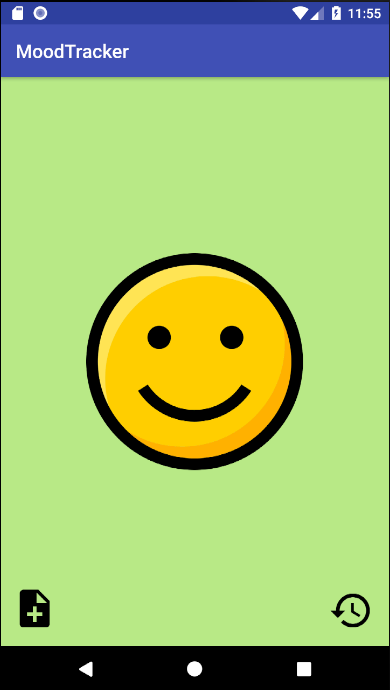
\includegraphics[width=.4\textwidth]{interface.png}
  \caption{Interface utilisateur}
  \label{interface}
\end{figure}
En bas de l'écran deux boutons sont disponibles :
\begin{itemize}
\item Le bouton en bas à gauche ouvre une boîte de dialogue permettant à l'utilisateur d'entrer un commentaire pour expliquer la raison de l'humeur choisie. Ce commentaire pourra être retrouvé dans l'historique. Sélectionne une autre humeur après avoir entrer un commentaire effacera ce dernier. 
\item Le bouton en bas à droite permet à l'utilisateur de voir l'historique des humeur enregistrées sur les sept derniers jours.
\end{itemize}

L'application peut s'utiliser en mode portrait ou en mode paysage selon les envies de l'utilisateur.

Pour la bonne construction de l'historique, l'application accède à la date de l'appareil. Donc si l'utilisateur change manuellement la date à une date antérieur, l'application affiche un message d'avertissement annonçant que le changement manuel de la date peut nuire à l'intégrité de l'historique\footnote{Seul les retours en arrière peuvent être détectés.}.

\section{Fonctionnalité de l'activité d'historique}

Lorsque l'utilisateur click sur le bouton d'accès à l'historique, un nouvel écran s'affiche sur lequel on peut voir les sept dernières humeur enregistrées de la semaine. Une petite icône apparaît les jours où l'utilisateur à laisser un commentaire. En cliquant sur la ligne où une icône apparaît, le commentaire enregistré apparaît en bas de l'écran  (voir la figure~\ref{historique1}).

\begin{figure}[!h]
  \centering
  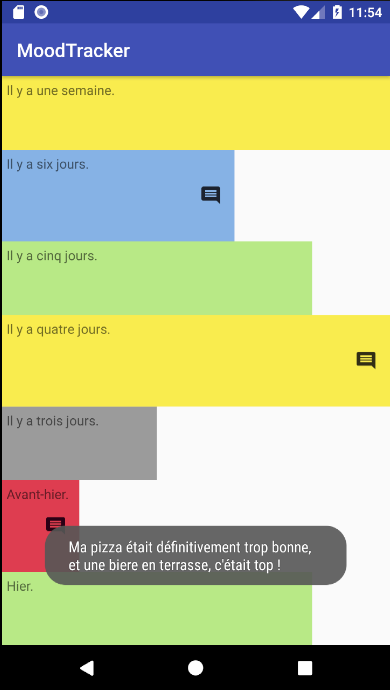
\includegraphics[width=.4\textwidth]{historique1.png}
  \caption{Exemple d'historique avec l'affichage d'un commentaire.}
  \label{historique1}
\end{figure}

L'application se comporte comme si elle enregistrait l'humeur courante à minuit.

S'il y a des jours où l'utilisateur ne se sert pas de l'application, ils seront indiquer dans l'historique avec un message disant que l'utilisateur n'a pas enregistré d'humeur ce jour-là. La figure~\ref{historique2} montre un exemple où l'utilisateur n'a pas utiliser l'application pendant deux jours.

\begin{figure}
  \centering
  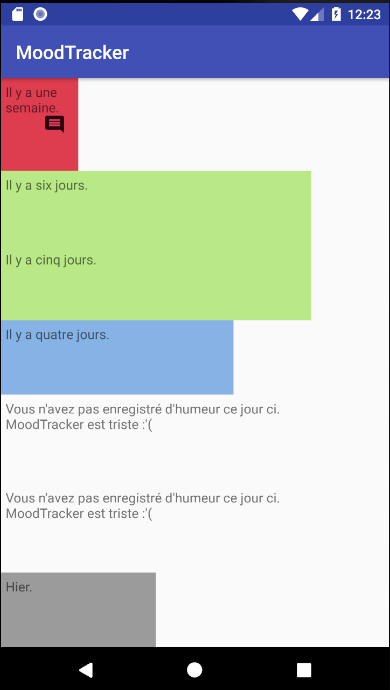
\includegraphics[width=.4\textwidth]{historique2.png}
  \caption{Exemple d'historique avec des jours manquants.}
  \label{historique2}
\end{figure}

Par défaut, lors de la première utilisation, l'historique n'affiche que des lignes indiquant qu'aucune humeur n'a été enregistrée pour le jour indiqué. Ces lignes disparaîtront au fur et à mesure que l'historique se mettra à jour avec les humeurs de l'utilisateur.


\end{document}
